\documentclass{article}
\usepackage{graphicx}
\usepackage[margin=1.5cm]{geometry}
\usepackage{amsmath}

\begin{document}
\twocolumn

\title{Friday warm-up: Forces II}
\author{Prof. Jordan C. Hanson}

\maketitle

\section{Memory Bank}

\begin{itemize}
\item $\vec{v} = \Delta \vec{x} / \Delta t$, the definition of velocity.
\item Newton's Second Law: $\vec{F}_{net} = m\vec{a}$. (The net external force on an object is equal to the mass of the object times the acceleration of the object).
\item $s = r\theta$ ... Let $s$ be the \textit{arc length} around a curve, with $r$ being the radius of curvature, and $\theta$ being angle between the initial and final position vectors.
\item $a_{\rm C} = v^2/r$ ... The centripetal acceleration given the speed $v$ around a circular path $r$.s
\end{itemize}

\section{Forces, II}

\begin{enumerate}
\item In Fig. \ref{fig:1}, a man with mass $m$ and weight $w$ stands on a scale in an elevator.  Which of the followinng is true, if the elevator is accelerating upwards?
\begin{itemize}
\item A: $w = mg$
\item B: $w < mg$
\item C: $w > mg$
\item D: $w = 0$
\end{itemize}
\item Suppose the man's mass is $60$ kg.  He is standing on a scale in an elevator that is \textit{accelerating upwards} at $0.2$ m/s$^{2}$.  What is the weight on the scale? \\ \vspace{1cm}
\item (a) Suppose a circular path as a radius of $10$ m.  If we travel 10 degrees around the circle, how far have we walked? (b) If we walk $200$ meters along a circular path, and determine that our direction changed by 90 degrees, what was the radius of curvature? \\ \vspace{1cm}
\item In Fig. \ref{fig:2}, a system moves in a circle with speed $v$.  The velocity changes direction by an angle $\Delta\theta$, as does the position.  It may be shown that this leads to \textit{centripetal acceleration}, $a_{\rm C}$.  (a) If a system is moving at 4 m/s around a curve with radius 0.25 m, what is $a_{\rm C}$? (b) What is $a_{\rm C}$ if $r = 1$ m? \\
\item Assume there is a force of friction $-f$ on $m_1$ in Fig. \ref{fig:3}.  Derive an expression for the acceleration of $m_2$.
\end{enumerate}

\begin{figure}
\centering
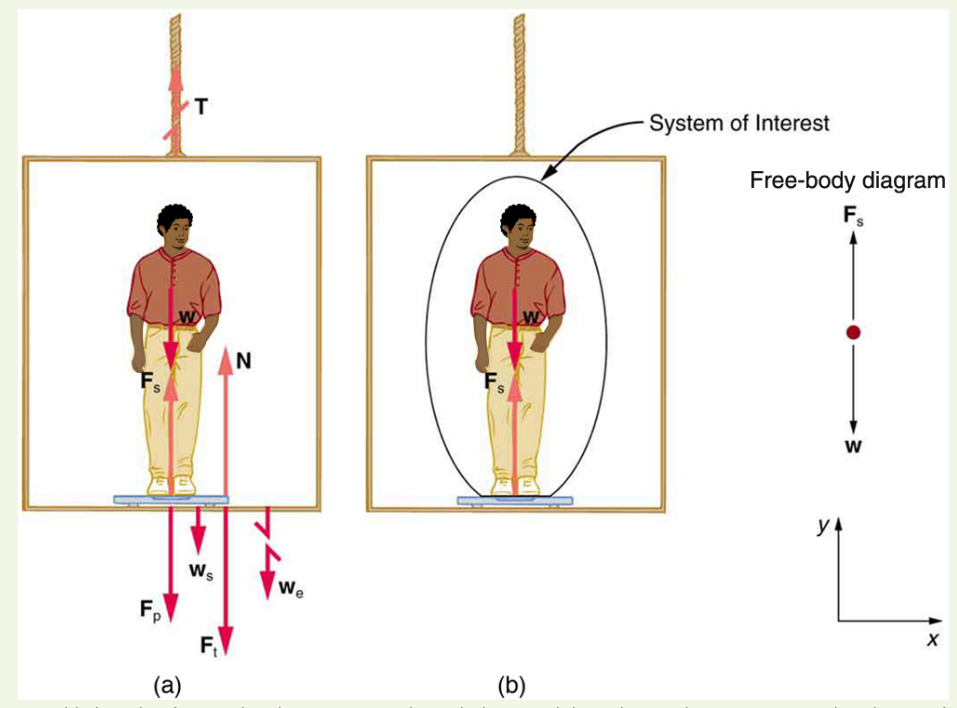
\includegraphics[width=0.2\textwidth,trim=13cm 0cm 0cm 0cm,clip=true]{elevator.png}
\caption{\label{fig:1} A person on a scale in an elevator.}
\end{figure}

\begin{figure}
\centering
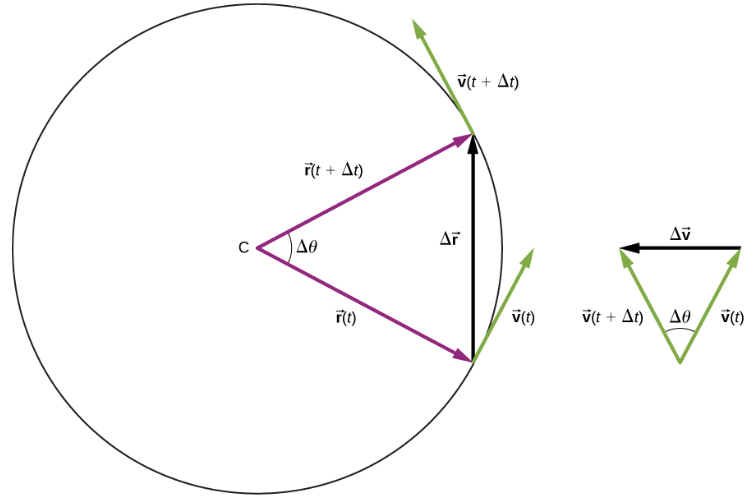
\includegraphics[width=0.3\textwidth]{figures/circle.png}
\caption{\label{fig:2} Uniform circular motion.}
\end{figure}

\begin{figure}
\centering
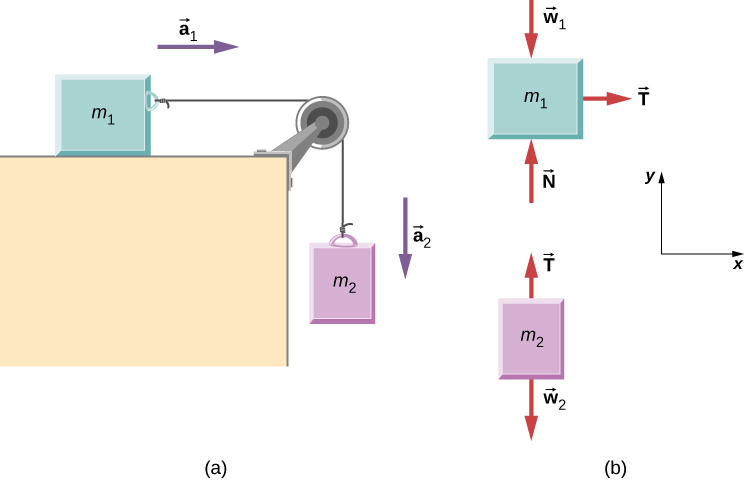
\includegraphics[width=0.3\textwidth]{figures/blocks.jpg}
\caption{\label{fig:3} Friction acts on block $m_1$ and gravity acts on $m_2$.}
\end{figure}

\end{document}
